\PassOptionsToPackage{bookmarks=false}{hyperref}
\documentclass[conference,final,a4paper]{IEEEtran}
\usepackage[bookmarks=false]{hyperref}

\hypersetup{
            pdftitle={A Robust Goal Programming Framework For Transfer Pricing Risk Hedging},
            pdfborder={0 0 0},
            breaklinks=true}
\urlstyle{same}  % don't use monospace font for urls

%\setcounter{secnumdepth}{0}

\usepackage{graphicx}
\usepackage{amsmath,mathtools}
\usepackage{tikz}
\usepackage{amsfonts}
\usepackage{cite}
\usepackage{booktabs}
\usepackage{drawstack}

\usetikzlibrary{shapes.geometric, arrows}
\tikzset{
  font={\fontsize{6pt}{12}\selectfont}}

\providecommand{\tightlist}{%
  \setlength{\itemsep}{0pt}\setlength{\parskip}{0pt}}

\renewcommand{\thesection}{\roman{section}}

\hyphenation{op-tical net-works semi-conduc-tor}

\begin{document}

\title{A Robust Goal Programming Model For Transfer Pricing Risk Hedging: Preliminary Results}

\author{
\IEEEauthorblockN{1\textsuperscript{st} Marco Repetto}
\IEEEauthorblockA{\textit{Department of} \\
\textit{Economics, Management and Statistics}\\
\textit{University of Milan-Bicocca}\\
Milan, Italy\\
m.repetto1@campus.unimib.it}
\and
\IEEEauthorblockN{2\textsuperscript{nd} Davide La Torre}
\IEEEauthorblockA{\textit{Dubai Business School} \\
\textit{University of Dubai}\\
Dubai, UAE \\
dlatorre@ud.ac.ae}
\textit{and}\\
\IEEEauthorblockA{\textit{Department of Economics,} \\
\textit{Management, and Quantitative Methods} \\
\textit{University of Milan}\\
Milan, Italy \\
davide.latorre@unimi.it}
\and
\IEEEauthorblockN{3\textsuperscript{rd} Danilo Liuzzi}
\IEEEauthorblockA{\textit{Department of}\\
\textit{Economics and Management}\\
\textit{University of Cagliari}\\
Cagliari, Italy \\
danilo.liuzzi@unica.it}
}

\maketitle

\begin{abstract}
In the following paper it is proposed a model for controlling the Transfer Pricing risk of a Multinational Firm operating in different countries and that has a well-defined value chain spread across its different controlled companies. These types of agreements controlling such transactions generally take into account different type of objectives. Another problem arises by the process itself that may appear to be fairly deterministic; such simplistic assumption decays if the focus is placed on the general length of such agreements that tend to occupy a medium length planning horizon. Because of that, a Robust Multicriteria Transfer Pricing risk model is built, using the multi-objective capabilities of the Goal Programming approach and the uncertainty modeling features provided by the concept of Robust Optimization. The final result is a model in order to handle the possible worst-case scenarios in an environment of high uncertainty and mid to long-term planning.
\end{abstract}

\maketitle

\IEEEpeerreviewmaketitle


\hypertarget{introduction}{%
\section{Introduction}\label{introduction}}

From Apple scandals \cite{leswing18} to Starbucks boycott protests
\cite{campbell16} this decade will probably be remembered as
the period where the tax avoidance problem gained particular momentum
among people and scholars, making the Transfer Pricing (TP) one of the most questioned topic of all time. It's not enough to stress the fact that transfer pricing it's just a practice and not a bad one per se \cite{oecd15}. Such perspective on the transfer pricing practices has been also highlighted by recent studies \cite{klassen16}: most of time, as reported, the goal of the Decision Maker (DM) is to achieve a set of goals not just tax minimization. Because the risk associated with TP practices is something affecting multiple economic agents, in recent years the OECD addressed this problem and shed some light on hoe to operate in such environment \cite{oecd12}. Looking at the reference literature very few improvements have been made to model the risk exposure in a rigorous and analytical way. Therefore, the model proposed tries to embed the expertise made by scholars in the field of multiple objective programming proposing a model for addressing the TP risk affecting a multinational company, in condition of uncertainty aiming at a solution that is robust \cite{bertsimas03} to environmental changes.

\hypertarget{methods-used}{%
\section{Methods used}\label{methods-used}}
The Goal Programming (GP) \cite{charnes55} pertains to the field of Multicriteria Decision Analysis (MCDA). GP is a distance-based method that relies on minimizing a set of deviation variables which model the distance between achieved levels and goals. In this setting the DM can take into account the deviation of each objectives from its goal, and using some projection algorithms the DM can determine Pareto optimal solutions. In this paper, the choice was to use the Weighted Goal Programming (WGP), because it allows for major trade-offs between each and every objective. Its formulation will be generalized and explained in the further paragraph.
\begin{subequations}
The WGP formulation reads as following:
\begin{align}
    & \underset{\delta}{\text{minimize}} & & w(\delta) \label{wgpmin} \\
    & \text{subject to} & & f_i(x)+ \delta_i=b_i, \; \forall i \in N \label{wgpsoftgoal} \\
    & & & x\in F \label{wgphardgoal}\\
    & & & \delta\geq 0 \label{wgppositivity}
\end{align}
\end{subequations}
where the objective function in (\ref{wgpmin}) is based on the minimization of the deviations that measure the distance between the objectives and the goals stated in (\ref{wgpsoftgoal}). Equation (\ref{wgphardgoal}) models the presence of more abstract constraints. It is worth noticing that the classical WGP approach does not leave any room for any kind of uncertainty associated with both the coefficients and the goals. These kinds of scenarios are better handled by another type of approach called Robust Optimization (RO). RO builds on the philosophy worst-case analysis and such idea has been applied extensively in many fields, ranging from statistics \cite{huber64} to machine learning \cite{vapnik63}\cite{tibshirani96}. Accounting for the uncertainty of parameters in operational research revealed to be crucial in order to avoid sub-optimal solutions or even unfeasible ones \cite{ben-tal00}. In contrast with Stochastic Optimization (SO) \cite{dantzig55}, which assumes probabilistic modeling of the uncertainty; robust optimization rejects this assumption posing that parameters vary arbitrarily in known bounded sets, called the uncertainty sets \cite{soyster73}. RO gained momentum in recent years thanks to the extended work of Ben-Tan and Nemirovski \cite{ben-tal97}\cite{ben-tal98}\cite{ben-tal99}.
\begin{subequations}
The robust formulation of a general programming model is:
\begin{align}
    & \underset{x}{\text{minimize}} & & f(x) \label{rpmin} \\
    & \text{subject to} & & g(x)=\chi(\xi), \; \xi \in \Xi \label{rpcon} \\
\end{align}
\end{subequations}

where in this case the single goal minimizes the cost function $f(x)$ depending upon the decision variable $x$, given a set of feasible uncertainty regions denoted by $\chi(\xi)$. Here the concept of uncertainty sets, denoted by $\Xi$, is extended to embed an area in which the DM will find its optimal solution. Of course, the feasible uncertainty regions can be $n$, where $n=1...+\infty$. In this approach, the more the uncertainty regions we consider the stricter becomes our solution. That's why the RO approach is said to be ``conservative'', even though in some case it may turn out to be not conservative at all when compared with SO \cite{ben-tal09}. The RO problem shown above has two major drawbacks, namely: (i) it does not include any measure of robustness which the DM can act on, and (ii) it does not allow (by design) to consider multiple objectives. A hybrid approach that tries to fix both of these problems affecting early stage RO formulations
was originally developed by Kuchta \cite{kuchta04}. In this formulation, the
robust tuning parameter is played by \(r\) where \(r=0...n\) given \(n\)
the number of parameters subjected to uncertainty.
\begin{subequations}
The compact formulation of a robust goal programming model reads as:
\begin{align}
    & \underset{\delta}{\text{minimize}} & & w(\delta) \label{wrgpmin} \\
    & \text{subject to} & & f_i(x) + \sum_{j=1}^{Q}p_{ij} + r_iz_i + \delta_i = b_i, \forall i \in N  \label{wrgpsoftgoal} \\
    & & & z_i + p_{ij} \geq g_{ij}(x), \forall i \in N , \forall j \in Q \label{wrgptuning} \\
    & & & x\in F \subseteq \mathbb{R}^{s} \label{wrgphardgoal} \\
    & & & \delta_i, p_{ij}, z_i \in \mathbb{R}^{+} \label{wrgppositivity}
\end{align}
\end{subequations}
The deviations in Equation (\ref{wrgpmin}) are weighted using the function $w$. It is worth noticing that in this formulation the tuning parameter that permits to adapt the level of robustness - sometimes referred to as the price of robustness \cite{bertsimas04} - is represented by \(r\), whereas Equation (\ref{wrgphardgoal}) models the presence of more abstract constraints. The formulation proposed by Kuchta was used by Ghahtarani and Najafi in the field of portfolio optimization \cite{ghahtarani13} where uncertainty affected the parameters related to portfolio selection resulting in a solution with an increased conservatism as well as its price of robustness.

\pagebreak

\hypertarget{transfer-pricing}{%
\subsection{Transfer Pricing Policies}\label{the-model}}
\begin{figure}
\centering
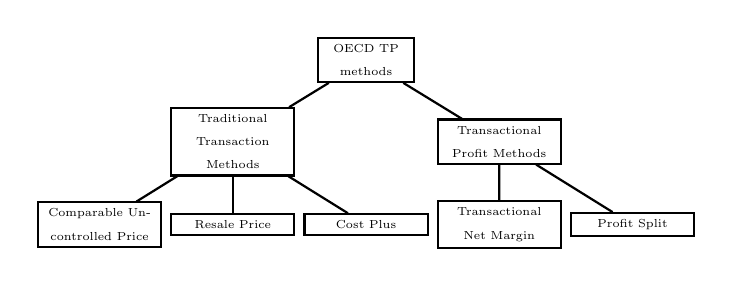
\begin{tikzpicture}[thick, every node/.style={scale=0.7}]
  \matrix [column sep=1mm, row sep=3mm] {
    & &
  \node (yw) [draw, shape=rectangle,text width=1.5cm,align=center] {OECD TP methods}; &
  & \\
  &
   \node (d1) [draw, shape=rectangle,text width=2cm,align=center] {Traditional Transaction Methods}; & &
  \node (d2) [draw, shape=rectangle,text width=2cm,align=center] {Transactional Profit Methods}; & \\
  \node (we) [draw, shape=rectangle,text width=2cm,align=center] {Comparable Uncontrolled Price}; &
  \node (wf) [draw, shape=rectangle,text width=2cm,align=center] {Resale Price}; &
  \node (wg) [draw, shape=rectangle,text width=2cm,align=center] {Cost Plus}; &
  \node (pu) [draw, shape=rectangle,text width=2cm,align=center] {Transactional Net Margin}; &
  \node (pl) [draw, shape=rectangle,text width=2cm,align=center] {Profit Split}; \\
};
\draw[-, thick] (d1) -- (we);
\draw[-, thick] (yw) -- (d1);
\draw[-, thick] (yw) -- (d2);
\draw[-, thick] (pu) -- (d2);
\draw[-, thick] (d1) -- (wg);
\draw[-, thick] (d1) -- (wf);
\draw[-, thick] (d2) -- (pl);
\end{tikzpicture}
\caption{TP methods in the OECD guidelines.} \label{fig:tp-m}
\end{figure}

Generally, Multinational Entities (MNE) subject to TP legislative burden tend to act proactively promoting agreements that bind the counterparts belonging to the same group for particular value-related process, in these agreements it is possible to identify different aspects: (i) the counterparts; (ii) the role of the counterparts; (iii) the remuneration of the counterparts; (iv) auxiliary clauses. The aspect of remuneration is crucial in these policies because may lead tax avoidance conducts. In the best practices provided by the OECD\cite{oecd17} several methods are proposed to cope with this aspect as presented in Figure \ref{fig:tp-m}. In the case under analysis we excluded the Traditional Transaction Methods because of a lack of comparable transactions involving the MNE and other third parties unrelated companies. Therefore the choice was to opt for Transactional Profit Methods. The Transactional Net Margin Method (TNMM) is based on the examination of the net profit relative to an appropriate base (e.g. costs, sales, assets) that a local entity realizes from a controlled transaction (or in our case to the entity itself). In order to achieve this is necessary to identify which Profit Level Indicator to choose; this is an important choice that has to be made taking into account the functional characterization of such entity. The main PLIs used by the practitioners are: Return on Sales (ROS), Full Cost Mark-up (FCMU), Return on Asset (ROA) and Return on Investment (ROI).

\hypertarget{the-model}{%
\section{The Model}\label{the-model}}
When dealing with the setting of the transfer prices, the DM faces a series of choices that most of the times conflict with each other, ranging from management profitability requirements to greedy tax minimization, hence a GP model has been chosen. Apart from the number of objectives considered a key role is played by the dynamics of the environment in which such decisions are taken, such environment tends to be influenced by a certain degree of uncertainty, and therefore the TP policies have to be robust in the sense that has to account for that uncertainty. The model that is going to be presented tries to cope with several
objectives coming from different vision of the company that ranges from
greedy tax minimization to management profit achievement.

\begin{subequations}
The deterministic WGP model formulation reads as:
\begin{align}
    & \underset{\delta^+,\delta^-}{\text{minimize}} & & \sum^{N}_{i=1}w_i(\delta^+_i + \delta^-_i) & \label{dm_obj} \\
    & \text{subject to} & & n\cdot \sum^{Q}_{j=1}(x_j\cdot t_j) - \prescript{t}{}{\delta^+}  =\overset{\star}{t} & \label{dm_tax} \\
    & & & n\cdot \frac{x_j}{b_j} - \prescript{m}{}{\delta^+_j} + \prescript{m}{}{\delta^-_j} = m_j, & \forall j \in Q \label{dm_median} \\
    & & & {x_j} - \prescript{g}{}{\delta^+_j} + \prescript{g}{}{\delta^-_j} = g_j, & \forall j \in Q \label{dm_management} \\
    & & & \sum^{Q}_{j=1} c_j(x_j) \geq p & \label{p_l} \\ 
    & & & \sum^{Q}_{j=1} c_j(x_j) \leq p + \Delta & \label{p_u} \\
    & & & n\cdot \frac{x_j}{b_j} \geq l_j, & \forall j \in Q \label{l_q} \\
    & & & n\cdot \frac{x_j}{b_j} \leq u_j, & \forall j \in Q \label{up_q}\\
    & & & \delta^+_i,\delta^-_i,x_j\geq 0  & \forall i \in N, \quad \forall j \in Q
\end{align}
\end{subequations}

Where the three types of deviational variables (highlighted by \(^t\),
\(^m\), \(^g\)) belong to main objectives described below. Equation (\ref{dm_tax}) refers to the tax minimization: in such objective the goal is to penalize any positive deviation in order to achieve the target tax liability level decide a priori by the management in this case $\overset{\star}{t}$ has to be intended as the absolute value of tax expenses that MNE would like to pay whereas the left hand side represent the current tax liability identified as:
  $$
  n\cdot \sum^{Q}_{j=1}(x_j\cdot t_j)  = \text{EBIT} \cdot \text{Tax Rate} = \text {Tax Liability} 
  $$
  Equation (\ref{dm_median}) refers to the TNMM goal for the net profit indicator to be in line with the median of a particular set of independent companies $m_j$ performing similar functions, whereas the left hand side represents the Earnings Before Interest and Taxes over the applicable base defined by TNMM in other terms:
  $$
  n\cdot \frac{x_j}{b_j} = \frac{\text{EBIT}_j}{\text{BASE}_j} \quad j \in Q \quad b = \begin{bmatrix} \text{Return On Sales} \\ \text{Return On Assets} \\ \vdots \end{bmatrix}
  $$
  Equations (\ref{l_q}) and (\ref{up_q}) represent the lower and upper quartile indicator boundary of the TNMM, as mentioned above this provide the range in which the tax risk result on a controllable level therefore these two equations are strictly related with the previous one. Equation (\ref{dm_management}) sets the management's objectives for each off-shore division in terms of margin per product. Equation (\ref{p_l}) and (\ref{p_u}) sets minimum and maximum price deviation accepted because of the TP policy. The decision variables \(x\) represent the margin of the product allocated to the j-th firm.

The model presented above was robustified against three
different factors: (i) uncertainty related to tax rate; (ii) uncertainty related to duties; (iii) uncertainty regarding the feasible range of compliance with the TNMM.

\begin{subequations}
The robust WGP model formulation reads as:
\begin{align}
& \underset{\delta^+,\delta^-}{\text{minimize}} \sum^{N}_{i=1}w_i(\delta^+_i + \delta^-_i)\\
& \text{subject to} \sum^{Q}_{j=1}(x_j t_j + \pi_{1,j})+ \prescript{t}{}{\rho} \prescript{t}{}{\zeta} - \prescript{t}{}{\delta^+}  =\overset{\star}{t} \\
& n\cdot \frac{x_j}{b_j}+\pi_{2,j}+ \prescript{m}{}{\rho} \prescript{m}{}{\zeta} - \prescript{m}{}{\delta^+} + \prescript{m}{}{\delta^-_j} = {m_j}, & \forall j \in Q \\
& {x_j} - \prescript{g}{}{\delta^+_j} + \prescript{g}{}{\delta^-_j}  = {g_j}, & \forall j \in Q \\
& \sum^{Q}_{j=1} c_j(x_j) + \pi_{3,j} + \prescript{t}{}{\rho} \prescript{g}{}{\zeta} \geq p \\
& \sum^{Q}_{j=1} c_j(x_j) + \pi_{3,j} + \prescript{t}{}{\rho} \prescript{g}{}{\zeta} \leq p + \Delta \\
& n\cdot \frac{x_j}{b_j} \geq {l_{j,u}}, \qquad  \forall j \in Q, \quad \forall u \in U \label{lquartile} \\
& n\cdot \frac{x_j}{b_j} \leq {u_{j,u}}, \qquad \forall j \in Q, \quad \forall u \in U \label{uquartile} \\
& \zeta_i + \pi_{ij} \geq \theta_{ij} x_{j},  \qquad \forall i \in N, \quad \forall j \in Q \\
& \delta^+_i,\delta^-_i,x_j\geq 0, \qquad \forall i \in N, \quad \forall j \in Q
\end{align}
\end{subequations}

The company data provided to the model were collected from a leading company in telecommunications and networking appliances with its production facility based in the Far-East and with the principal and distributional functions based in the European Union soil. Because of a matter of confidentiality, the data were anonymized, with this procedure the relevant functionalities of the model remained intact although preserving the corporate financial strategies. Conversely, the comparable companies' data used for the TNMM method application were obtained by ad-hoc business related databases such as Orbis \cite{orbis} provided by Bureau van Dijk a major publisher of business information, specialized in private company data. In the following table is given an overview of such data.

\begin{table*}[]
\centering
\caption{Entity specific data and goals.}
\label{es-goal}
\begin{tabular}{@{}lllllllllll@{}}
\toprule
ID & Function & Tax-Rate   & Variable Cost & Fixed Cost    & Duty & Management Goal & Lower Quartile & Median & Upper Quartile \\ \midrule
1  & manufacturer & 0.25  & 23.75 & 811800.0 & 0.15   & 3.2   & 0.04      & 0.08   & 0.14      \\
2  & distributor  & 0.30  & 11.3  & 35700.0  & 0.0    & 2.8   & 0.01      & 0.02   & 0.05      \\
3  & principal    & 0.125 & 16.8  & 171000.0 & 0.0    & 5.1   & 0.02      & 0.07   & 0.14      \\ \bottomrule
\end{tabular}
\end{table*}

The noise matrix \(\theta^{Q \times (N\cap N^0) }\) applied to the
coefficient was the following one:

\[ \mathbf{\Theta} =  \begin{bmatrix}
 0.0125 & 0.0750 & 0.0060 & 0.0120 & 0.0210 \\
 0.0300 & 0.0000 & 0.0012 & 0.0024 & 0.0060 \\
 0.0250 & 0.0000 & 0.0042 & 0.0147 & 0.0294 \\
 \end{bmatrix} \]

These have to be intended as the maximum shifts that each variable may
be subjected to. In both cases, namely with the corporate taxes and duties,
these shifts may be positive, whereas in case of the TNMM values such
shifts will be negative since a lower level of the test PLI will result
in a worst case scenario and not the other way around.

\hypertarget{model-deploy}{%
  \subsection{Model Deploy}\label{model-deploy}}
The deploy of the model was pursued through Julia\footnote{Version 1.0.3 (2018-12-18), built on GNU/Linux Fedora 29.} which is a high-level, high-performance dynamic programming language for technical computing\cite{bezanson17}. The full stack used for the deployment of the model was divided as such:
\begin{itemize}
\item Algebraic modelling stack: the formalization of the robust model was obtained by using JuMP\cite{dunning17}\cite{lubin15}, a modeling language for mathematical optimization embedded into Julia and for the implementation of the Lexicographic approach the vOptSolver\cite{xavier17} library was used.
\item Solvers stack: the solver stack was primarily divided into two solvers:
  \begin{itemize}
  \item COIN-OR\cite{heimer2003} Linear Programming solver: the interface was provided by the Clp.jl package embedded into the JuliaOpt library;
  \item GNU Linear Programming Kit: the interface was provided by the Julia GLPK module embedded into the JuliaOpt library.
  \end{itemize}
\end{itemize}

\hypertarget{results}{%
\section{Results}\label{results}}
Since the approach applied was a weighted one, it was performed a sensitivity analysis \cite{jones11} in order to test the possible achievable objectives and their trade-offs with respect to the weights. In the ternary plot depicted at Figure \ref{tern} are presented the various combinations of weights and the sum of the decisional variables. Such sensitivity was tested by assuming no robustness of the model (\emph{i.e.} $\rho = [0,0,0]$).

\begin{figure}
\centering
\includegraphics[width=3.0in]{figure/ternary.png}
\DeclareGraphicsExtensions.
\caption{Weight sensitivity ternary plot.}
\label{tern}
\end{figure}

From such Figure is worth noting the decrease in profit allocation in case of a greater tax liability concern, that is, a possible strategy to obtain less taxation is indeed given by allocating fewer resources to the controlled companies and consequently shrinking the price of the good. Conversely, other weighting schemes tend to not change the value of the objective function but just how the profits are allocated among the entities. However as emerged in the literature, the main goal of the agents setting the TP policy is not always a mere focus on achieving a lower tax burden but instead on be as compliant as possible with the best practices in order to avoid any tax-related risk. Therefore the choice was to give major importance to the second objective then leaving the other two, namely management goal and
tax liability minimization, the same importance. The robustness array identified with \(\rho\) was subjected to a sensitivity analysis, therefore a different set of elements where used
ranging form \(0\) to \(n\). The following graph indentifies the different margin distribution among the three entities.

\begin{figure}[]
\centering
\includegraphics[width=3in]{figure/Figure_1.png}
\DeclareGraphicsExtensions.
\caption{Rho permutations and objective function results.}
\label{last}
\end{figure}

\hypertarget{more-result}{%
  \subsection{More on results: a Lexicographic and Naive comparison}\label{conclusion}}

\begin{table}[]
\centering
\caption{Results comparison: Robust, Naive and Lexicographic.}
\label{res-comparison}
\begin{tabular}{@{}llll@{}}
\toprule
  Entity       & Robust & Naive & Lexicographic \\ \midrule
  Manufacturer & 1.67   & 1     & 0.99     \\ 
  Distributor  & 1.08   & 2.2   & 0.62     \\
  Principal    & 2.86   & 5.1   & 2.17     \\ \bottomrule
\end{tabular}
\end{table}

\begin{table}[]
\centering
\caption{Results comparison: feasibility.}
\label{fea-comparison}
\resizebox{\columnwidth}{!}{%
\begin{tabular}{@{}llllll@{}}
\toprule
  Indicator         & Robust & Naive & Lexicographic & Lower Bound & Upper Bound \\ \midrule
  Manufacturer PLI  & 0.0680 & 0.0407   & 0.0403     & 0.0460      & 0.1610            \\ 
  Distributor  PLI  & 0.0176 & 0.0359   & 0.0101     & 0.0112      & 0.0560            \\
  Principal    PLI  & 0.0423 & 0.0755   & 0.0321     & 0.0242      & 0.1694            \\ 
  Final Price       & 63.70  & 68.73    & 63.25      & 61.20      & 63.7        \\ \bottomrule
\end{tabular}
}
\end{table}

\begin{table}[]
\centering
\caption{Results comparison: deviations from the objective.}
\label{dev-comparison}
\resizebox{\columnwidth}{!}{%
\begin{tabular}{@{}lllllll@{}}
\toprule
  Entity       & \multicolumn{2}{l}{Robust} & \multicolumn{2}{l}{Naive} & \multicolumn{2}{l}{Lexicographic} \\
                        &$\delta^+$&$\delta^-$&$\delta^+$&$\delta^-$&$\delta^+$&$\delta^-$ \\ \midrule
  Tax Objective         & $163.33\%$ & -        & $277.32\%$ & -        & $69.99\%$ & - \\ 
  TNMM Objective        & -         & $97.36\%$ & -          & $6.18\%$ & - & $173.06\%$ \\
  Management Objective  & $49.46\%$  & -        & $25.23\%$  & -        & $65.95\%$ & - \\ \bottomrule
\end{tabular}
}
\end{table}

Because of the lack of any recent research\cite{merville1978} about the topic of MCDA applied to the field of TP it was worth to set up a rigorous experiment to prove the effectiveness of such work. Therefore the decision was to test the goodness of the model in comparison with two other types of approaches namely: (i) the Naive approach (DM chose at random), (ii) the Lexicographic approach (DM solves the Lexicographic Goal Program associated). The two approaches were compared with the model at its maximum robustness (\emph{i.e.} $\rho=[3,3,3]$), in such setting we could test the feasibility of the results obtained. At first sight, it is worth noting from Table \ref{res-comparison} how the allocation changed from one approach to another. In particular, the Lexicographic approach tended to distribute a considerably lower margin through the entities, this behavior is due to the fact that even when deviations are normalized the tax objective tends to shrink the overall profit distribution, such behavior is highlighted also in the weight sensitivity analysis depicted in Figure \ref{tern}. In Table \ref{fea-comparison} emerges clearly that the allocation as proposed in the previous table is not feasible for the Naive and the Lexicographic approach, in particular, a relatively low shift in the lower quartile can hardly compromise such allocations. Leaving aside the considerations about the feasible points is possible to compare the different objectives achieved by the different approaches by studying the under and over-achievement collected by the normalized deviational variables depicted in Table \ref{dev-comparison}.

\hypertarget{conclusion}{%
\section{Conclusion}\label{conclusion}}
The paper proposed a model for intercompany transaction pricing which complies with the legislation in terms of transfer pricing policies. Because of the number of conflicting objectives the best approach seemed to be the GP one. However, taking into account just the conflicting objectives do not leave any remedy to possible uncertainties arising from exogenous variables. Because of that, the concept of RO was introduced. The results were encouraging: the solution remains feasible even in case of shifts of the economic environment and this confirms that the GP in its robust counterpart can indeed be a sounding tool in the hands of professionals when setting their TP policies.

\bibliographystyle{plain}   % (uses file "plain.bst")

\bibliography{reference}

\end{document}

